\documentclass[DIV16,BCOR1cm,11pt,a4paper,fleqn,twoside,onecolumn,notitlepage]{scrreprt}

\makeatletter
\renewcommand\chapter{\par%
  \thispagestyle{plain}%
  \global\@topnum\z@
  \@afterindentfalse
  \secdef\@chapter\@schapter}
\makeatother

\usepackage{graphicx,subfig,color}
\usepackage{listings}
\definecolor{zebg}{rgb}{1,1,.8} %elfenbeinfarbig 
\usepackage{wrapfig}
\usepackage{float}
\setcapindent{0pt}
\usepackage{makeidx}
\usepackage{thumbpdf}

\usepackage{hyperref}
\hypersetup{pdftoolbar=true,
            pdfmenubar=true,
            pdfwindowui=true,   
%            pdffitwindow=true,
            pdfauthor={Deike Kleberg},
            pdftitle={CDI-pio Manual},
            pdfcreator={pdflatex + hyperref},
            pdfstartview=FitV,
%            pdfpagemode=FullScreen,
            a4paper,
            bookmarks=true,
            linkcolor=blue,
            citecolor=blue,
            urlcolor=blue,
            colorlinks=true}

\usepackage[all]{hypcap}
\usepackage{nameref}


\setlength{\parindent}{0pt} 

\newcommand{\CDI}{\bfseries\sffamily CDI}
\newcommand{\pio}{\bfseries\sffamily CDI-pio}

\newcommand{\tabbox}[1]{\parbox{11.5cm}{\rule{0pt}{1.1\baselineskip}#1\vspace{1ex}}}

\newcommand{\deflabel}[1]{\bf #1\hfill}
\newenvironment{deflist}[1]
{\begin{list}{}
{\settowidth{\labelwidth}{\bf #1}
\setlength{\parsep}{0mm}
\setlength{\itemsep}{1mm}
\setlength{\leftmargin}{\labelwidth}
\addtolength{\leftmargin}{\labelsep}
\renewcommand{\makelabel}{\deflabel}}}
{\end{list}}

\makeindex
\newcommand{\idxdotfill}{\ \dotfill \ }

\begin{document}

\title{{\pio}, {\CDI} with parallel I/O}
\author{Deike Kleberg, Uwe Schulzweida, Thomas Jahns and Luis Kornblueh\\
Max-Planck-Institute for Meteorology and Deutsches Klima Rechenzentrum\\
Project ScalES funded by BMBF}
\date{\today}
\maketitle

\tableofcontents
\listoffigures

\chapter{Introduction}
The scalability of Earth System Models (ESMs) is the leading target of the 
\href{http://www.dkrz.de/Klimaforschung/dkrz-und-klimaforschung/infraproj/scales
}{ScalES}
project, in particular with regard to future computer development. Our work  
focuses on overcoming the I/O bottleneck.  The 
\href{https://code.mpimet.mpg.de/projects/cdi}{Climate Data Interface} ({\CDI}) is a 
sophisticated data handling library of 
the Max-Planck-Institute for Meteorology with broad acceptence in the 
community. 
\begin{wrapfigure}{r}{.4\textwidth}
\vspace{-10pt}
\centering
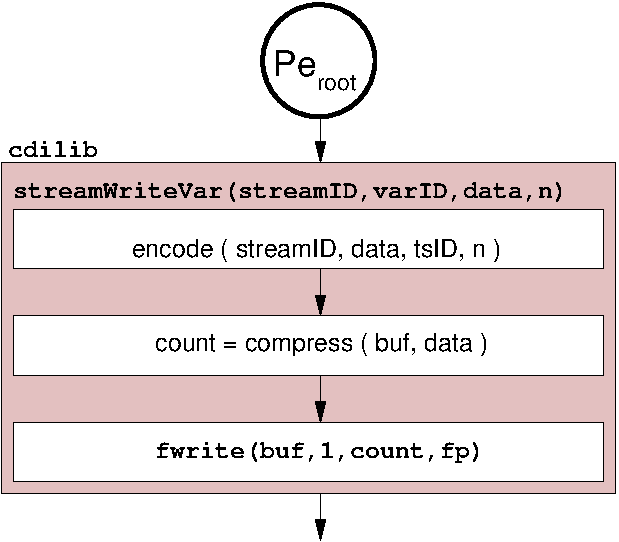
\includegraphics[scale=0.5]{../graphics/serial.pdf}
\vspace{-10pt}
\caption{{{\CDI} {\tt streamWriteVar}}}
\vspace{-10pt}
\end{wrapfigure}
Its I/O is carried out synchronously relative to the model calculation. 
We have decided to parallelize the file writing with the {\CDI}, because of the 
great benefit for many ESMs.
\smallskip 
 
We analyzed 
some HPC systems concerning the impact of their architecture, filesystem and 
MPI implementation on their I/O performance and scalability. The investigation 
delivered a large spectrum of results. As a consequence, 
we introduce different modes of low level file writing. The tasks 
of the I/O processes, which are now decoupled from the model calculation, are split.
We destinguish into collecting the data, encode, compress 
and buffer it on one side and writing the data to file on the other. The extension 
of the {\CDI} with parallel writing ({\pio}) provides five different I/O modes 
making use of this role allocation. The modulation of I/O mode, numbers and 
location of processes with the best performance on a 
special machine can be determined in test runs. 
\smallskip  

On some systems it is impossible to write from different physical nodes to one 
file. Taking the architectural structures into consideration we made a key 
pillar for the design of {\pio} from the distribution of I/O processes and files 
on physical nodes. If the I/O processes are located on different physical nodes, 
the {\tt MPI} communicator for the group of I/O processes is split and each 
subgroup gets a loadbalanced subset of the files to write. On some machines 
this approach increases the throughput remarkably.
\smallskip 

The application programming interface of the {\CDI} is kept untouched, 
we introduce only a few indispensable functions and encapsulate the other 
developments inside the library. The models have to eliminate the special 
position of the root process with respect to file writing. All model processes 
``write'' their chunk of the decomposed data and save the time former needed 
for gathering and low level writing. 

\chapter{I/O stages in the program flow}
With the concept of I/O stages in the model program flow {\pio} meets two of the 
main requirements for asynchronous I/O with the {\CDI}: The consistency of the 
resources on {\tt MPI} processes in different groups and the minimization of the 
communication. The program flow is divided in three stages:
\smallskip

\hspace*{4mm}\begin{minipage}[]{15cm}
\begin{deflist}{\tt STAGE\_DEFINITION \ } 
\item[{\htmlref{\tt STAGE\_DEFINITION}{STAGEDEFINITION}}]
The {\CDI} resources have to be defined.
\item[{\htmlref{\tt STAGE\_TIMELOOP}{STAGETIMELOOP}}]
Data can be moved from the model to the collecting I/O server.
\item[{\htmlref{\tt STAGE\_CLEANUP}{STAGECLEANUP}}]
The {\CDI} resources can be cleaned up.
\end{deflist}
\end{minipage}
\bigskip

A listing of an example program built up of control (\ref{control}) and 
model run (\ref{model}) in chapter \nameref{modules} clearifies the program flow.

\section{Define {\CDI} resources: {\tt STAGE\_DEFINITION}}
\index{STAGEDEFINITION@{\tt STAGE\_DEFINITION}}
\label{STAGEDEFINITION}
{\tt STAGE\_DEFINITION} is the default stage and starts with a call to 
{\htmlref{pioInit}{pioInit}}. During this stage, the {\CDI} resources have to 
be defined. Trying to write data with {\CDI} {\tt streamWriteVar} will lead to an 
error and abort the program. The stage is left by a call to 
{\htmlref{pioEndDef}{pioEndDef}}. After leaving, any call to a {\CDI} 
subprogramm XXX{\tt def}YYY will lead to an error and abort the program. 

\section{Writing in parallel: {\tt STAGE\_TIMELOOP}}
\index{STAGETIMELOOP@{\tt STAGE\_TIMELOOP}}
\label{STAGETIMELOOP}
{\tt STAGE\_TIMELOOP} starts with a call to {\htmlref{pioEndDef}{pioEndDef}}. 
Invocations to {\CDI} {\tt streamClose},\\
 {\tt streamOpenWrite}, 
{\tt streamDefVlist} and {\tt streamWriteVar} effect the local {\CDI} resources 
but not the local file system. The 
calls are encoded and copied to a {\tt MPI} window buffer. 
You can find a flowchart of one timestep in figure~\ref{timestep}. 
{\tt streamClose}, {\tt streamOpenWrite} and {\tt streamDefVlist} have 
to be called 
\begin{itemize}
\item only for an already defined stream/vlist combination,
\item in the suggested order, 
\item at most once for each stream during one timestep and 
\item before any call to {\tt streamWriteVar} in that timestep. 
\end{itemize}
% todo stream calls collective?
All four {\CDI} stream calls require that the model root process participates. 
Disregards to this rules will lead to an error and abort the program. The 
implication also holds for attempts to define, change or delete {\CDI} resources 
during {\tt STAGE\_TIMELOOP}. Therefor it is necessary to switch stages before 
cleaning up the resources. A call to 
{\htmlref{pioEndTimestepping}{pioEndTimestepping}} closes 
{\tt STAGE\_TIMELOOP}. 

\section{Cleanup {\CDI} resources: {\tt STAGE\_CLEANUP}}
\index{STAGECLEANUP@{\tt STAGE\_CLEANUP}}
\label{STAGECLEANUP}
{\tt STAGE\_CLEANUP} is launched by invoking 
{\htmlref{pioEndTimestepping}{pioEndTimestepping}}. In this stage, the {\CDI}
resources can be cleaned up. Trying to write data with {\CDI} 
{\tt streamWriteVar} will now lead to an error and abort the program. 

\section{The namespace object}
\index{namespace}
\label{namespace}
For some models the concept of stages is to narrow. In order to meet this 
requirement we introduce namespaces. A namespace 
\begin{itemize}
\item has an identifier,
\item is mapped to a {\CDI} resource array,
\item indicates, if the model processes write locally or remote,
\item has an I/O stage and
\item is the active namespace or not.
\end{itemize}
A call to {\htmlref{pioInit}{pioInit}} initializes the namespace objects with two 
of the arguments given by the model processes, the number of namespaces to be 
used and an array 
indicating if they obtain local or remote I/O. Invoking 
{\htmlref{pioNamespaceSetActive}{pioNamespaceSetActive}} switches the namespace 
so that subsequent {\CDI} calls operate on the resource array mapped to the 
chosen namespace. The namespaces are destroyed by 
{\htmlref{pioFinalize}{pioFinalize}}. If the model uses the {\CDI} serially, 
exactly one namespace supporting local writing is a matter of course. To save 
overhead, it is preferable to work with one namespace.


\chapter{Modes of low level writing}
The I/O performance and scalability of a supercomputer depends on the combination 
of the hardware architecture, the filesystem and the {\tt MPI} implementation. We 
made testruns on several machines invoking {\tt MPI\_File\_iwrite\_shared}, the 
obvious way of parallel file writing.  
Especially on the IBM Blizzard, naturally in our primary focus, the 
benchmark programs achieved surprisingly poor results. 
Accordingly the {\CDI} has to provide possibilities to write files in parallel 
using {\tt POSIX IO}.
The tasks formerly carried out by the root process are split into the subtask 
gather, encode and compress on one side and write the files on the other. The 
variable partition of these subtasks in the group of I/O server led us to five 
modes of low level writing. 
{\pio} is backwards compatible due to the differentiated behavior of the {\CDI} 
calls {\tt streamClose}, {\tt streamOpenWrite}, {\tt streamDefVlist}
and {\tt streamWriteVar} on model side, depending on local writing and I/O stage. 
 The {\tt stream} functions were primarily written for low level file writing, 
as a matter of course 
 also the collecting I/O processes invoke them. This makes the I/O modes to 
another key to the program flow of the {\CDI} stream calls.
\begin{figure}[H]
%\vspace{-10pt}
\centering
\subfloat[Legend]{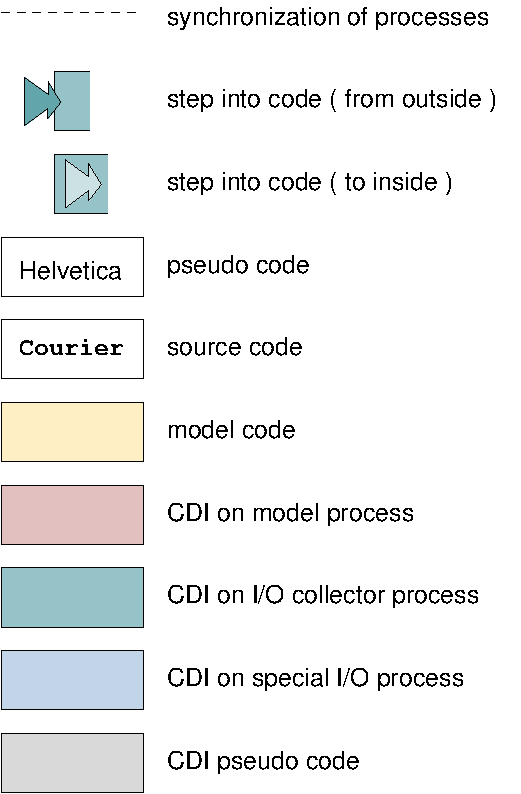
\includegraphics[scale=0.48]{../graphics/legend.pdf}}
\hspace{40pt}
\subfloat[Pseudo code encodeNBuffer]
{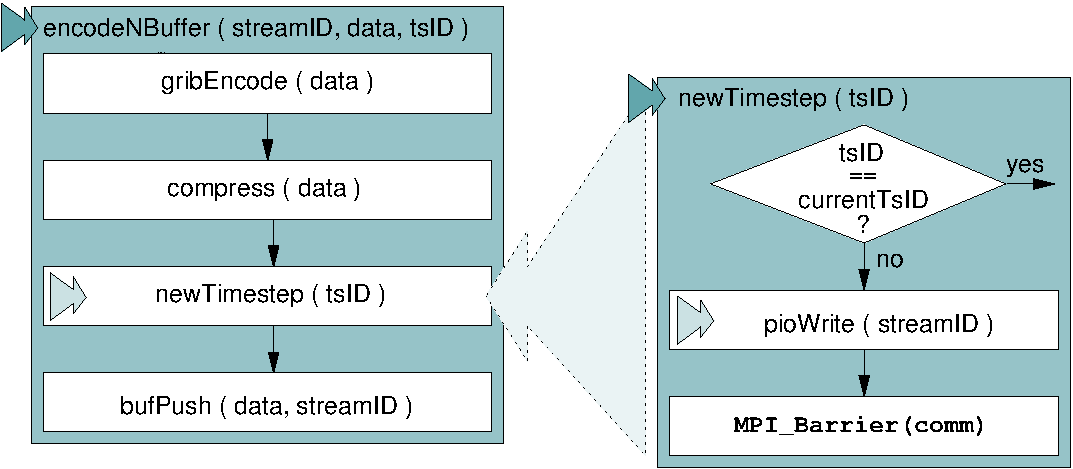
\includegraphics[scale=0.52]{../graphics/encodeNBuffer.pdf}}
%\vspace{-10pt}
\caption {Legend and pseudo code encodeNBuffer}
\index{legend}
\index{encodeNBuffer}
\label{legend}	
%\vspace{-10pt}
\end{figure}
On the I/O processes 
the excecution of the subprogram {\tt streamWriteVar} is controlled by the I/O 
 modes. To clearify the functioning we use pseudo code and
flowcharts as you can see in figure~\ref{legend}. 
The command 
\texttt{encodeNBuffer} abstracts the encoding, compressing and buffering
of the data for a variable. The data in a 
{\tt GRIB} file may not be mixed by time, so we need a command \texttt{newTimestep} 
to manage the flushing of the output buffers on the I/O server side. To 
achieve this, a \texttt{MPI\_Barrier} is used. 


\bigskip

I/O modes provided by {\pio}:

\bigskip

\hspace*{4mm}\begin{minipage}[]{15cm}
\begin{deflist}{\tt PIO\_FPGUARD\ } 
\item[{\htmlref{\tt PIO\_NONE}{PIONONE}}] 
one process collects, transposes, encodes, compresses, buffers and writes using 
{\tt C} {\tt fwrite}.
\item[{\htmlref{\tt PIO\_MPI}{PIOMPI}}] 
all processes collect, transpose, encode, compress, buffer and write using 
{\tt MPI\_File\_iwrite\_shared}.
\item[{\htmlref{\tt PIO\_ASYNCH}{PIOASYNCH}}]
one process writes the files using low level 
{\tt POSIX\_AIO}, the others collect, transpose, encode, compress and buffer.
\item[{\htmlref{\tt PIO\_FPGUARD}{PIOFPGUARD}}]
one process guards the fileoffsets, all others 
collect, transpose, encode, compress and write using {\tt C} {\tt fwrite}.
\item[{\htmlref{\tt PIO\_WRITER}{PIOWRITER}}]
one process writes the files using {\tt C} {\tt fwrite}, 
the others collect, transpose, encode, compress and buffer.
\end{deflist}
\end{minipage}


\section{{\tt PIO\_NONE}: $1$ process collects and writes using {\tt POSIX IO}}
\index{PIONONE@{\tt PIO\_NONE}}
\label{PIONONE}

The I/O mode {\tt PIO\_NONE} can only be run with one I/O process per physical 
node. This 
process collects, encodes, compresses, buffers and writes the data to the files 
attributed 
to his node. For low level file writing the {\tt C} standard \texttt{fwrite} 
is used. The advantages 
in comparison with the former serial writing are that the writing is done 
asynchronous with respect to the calculation and that the data is buffered. In 
addition it can be executed in parallel spread over physical nodes.

\begin{figure}[H]
\vspace{-10pt}
\centering
\subfloat[{\tt PIO\_NONE}]{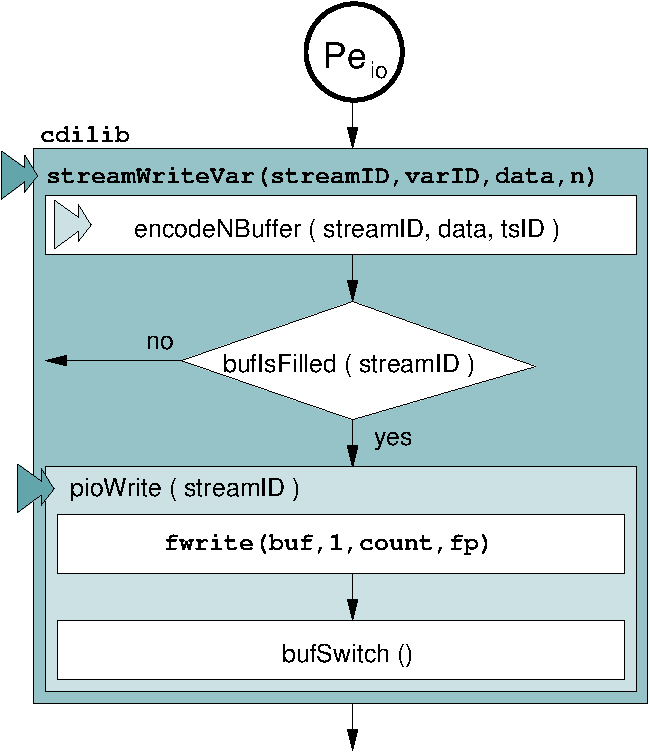
\includegraphics[scale=0.5]{../graphics/pio_none.pdf}}
\hspace{50pt}
\subfloat[{\tt PIO\_MPI}]{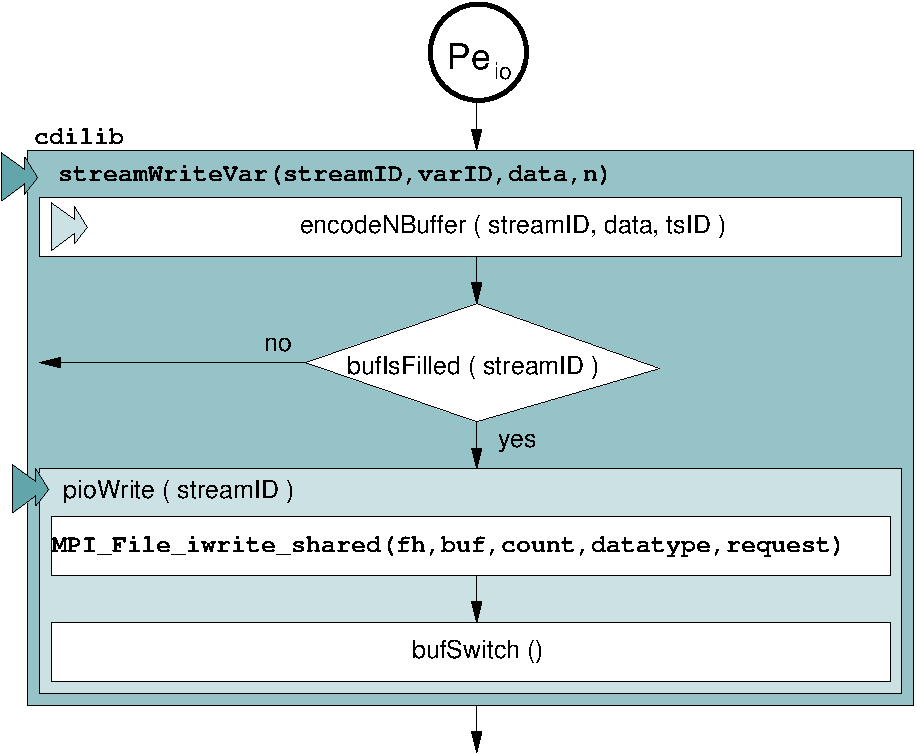
\includegraphics[scale=0.5]{../graphics/pio_mpi.pdf}}
\vspace{-10pt}
\caption {{\tt PIO\_NONE} and {\tt PIO\_MPI}}	
\vspace{-5pt}
\end{figure}

\section{{\tt PIO\_MPI}: $n$ processes collect and write using {\tt MPI IO}}
\index{PIOMPI@{\tt PIO\_MPI}}
\label{PIOMPI}

Data access using {\tt MPI} is the straight forward way to parallel file 
manipulation. With \\
{\tt MPI\_File\_iwrite\_shared} the processes have a shared 
file pointer available. The function is nonblocking and split collective. Like 
{\htmlref{\tt PIO\_NONE}{PIONONE}} the I/O mode {\tt PIO\_MPI} has no division 
of task within the I/O group, all processes collect, encode, compress, buffer and 
write to file. Writing in this I/O mode strongly depends on the {\tt MPI} 
implementation, the buffers used internally are of major importance for the 
performance of writing.

\section{{\tt PIO\_WRITER}: $n - 1$ processes collect and $1$ writes using 
{\tt POSIX IO}}
\index{PIOWRITER@{\tt PIO\_WRITER}}
\label{PIOWRITER}

\begin{figure}[H]
\vspace{-10pt}
\centering
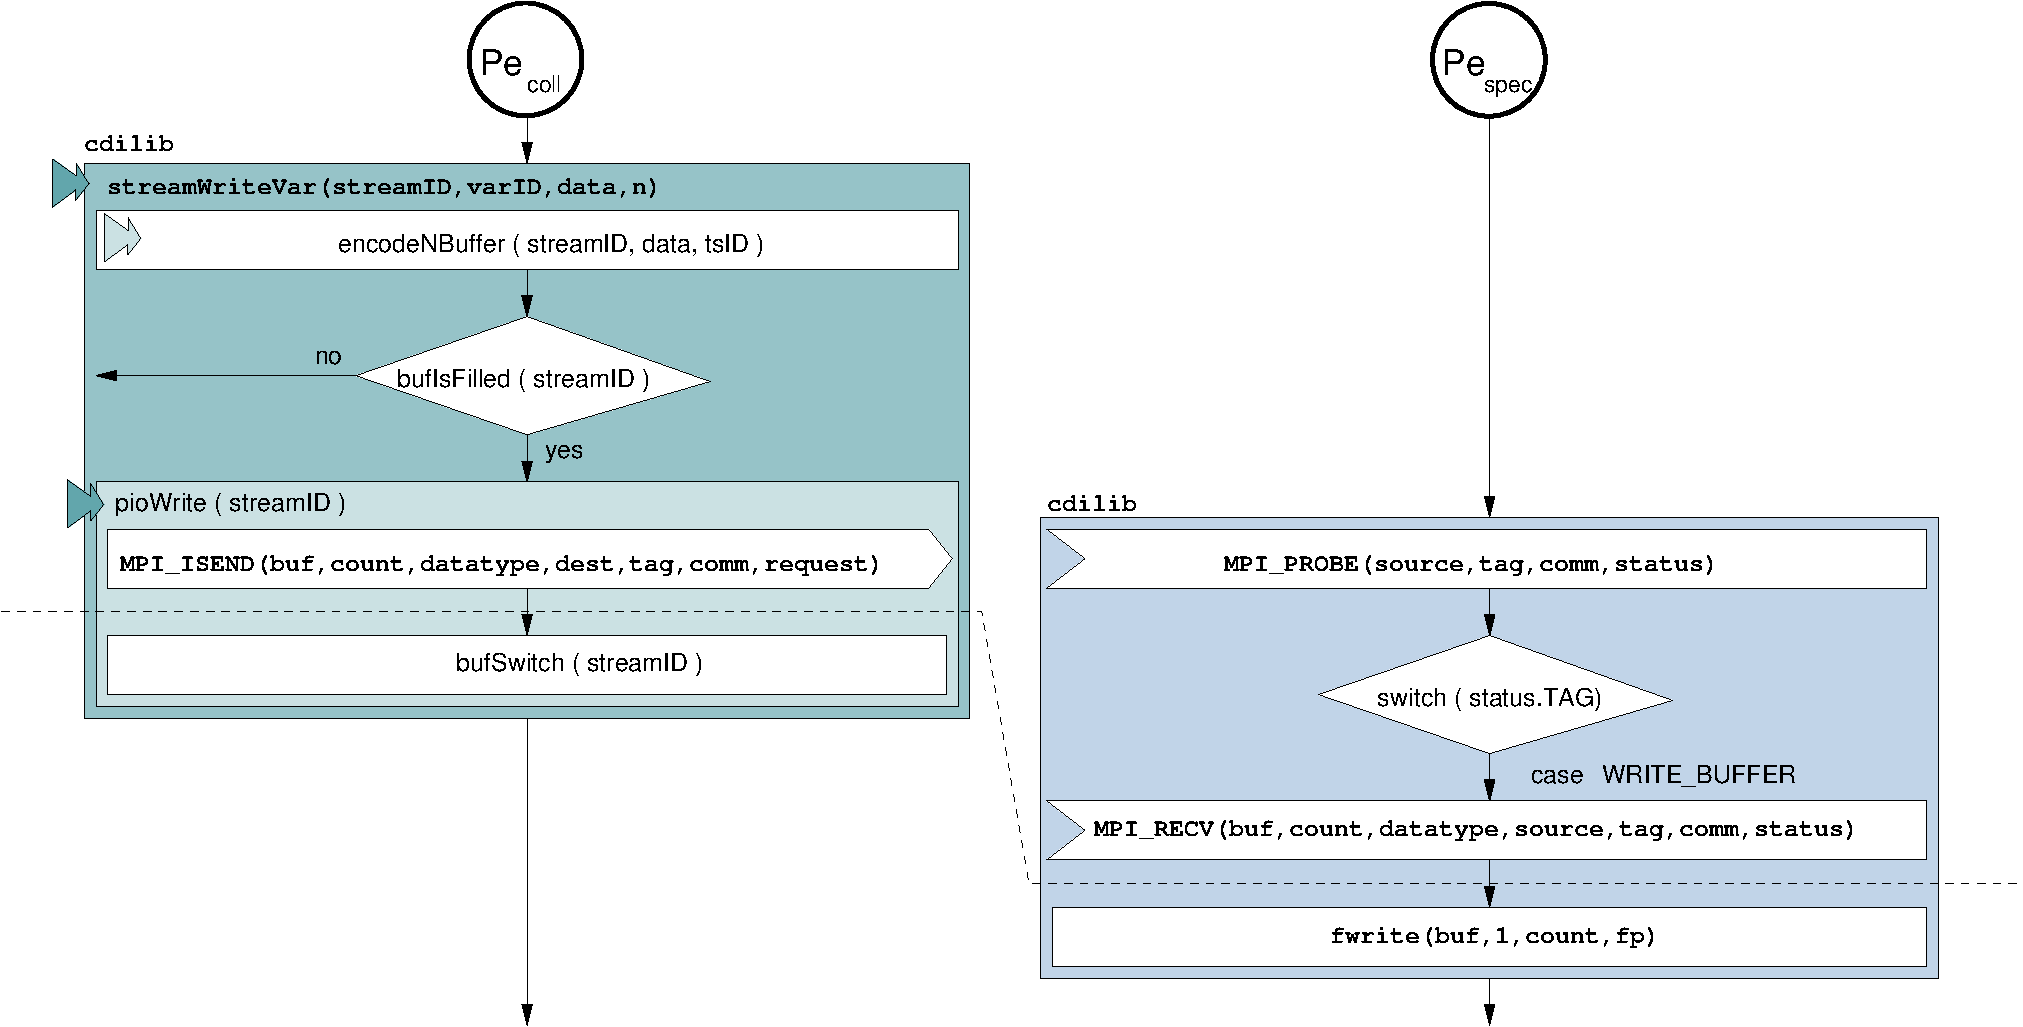
\includegraphics[scale=0.47]{../graphics/pio_writer.pdf}
\caption{{\tt PIO\_WRITER}}
\vspace{-10pt}
\end{figure}
If the I/O mode {\tt PIO\_WRITER} is chosen, the subtasks of writing are split
between the I/O processes. Just one process per physical node does the
low level writing  while the others collect, encode, compress and buffer 
the data. The writer is the process with the highest rank within the
I/O group on one physical node. Originating from {\htmlref{\tt pioInit}{pioInit}} 
he invokes a
backend server function, which he does not leave until he received messages from 
all  
collecting I/O processes to finalize.  A collector gets data from the calculating 
model processes via {\tt MPI RMA} communication, and, after encoding and
compressing it, pushes it to a double buffer. If the buffer is filled,
the contained data is send via \texttt{MPI\_Isend} to the writer, the 
collector
switches to the other buffer and continues his job. Before sending the
data he has to wait for a potentially outstanding
\texttt{MPI\_Request}. This might happen if the writer or the buffers
used by {\tt MPI} are overcommited and indicates that the ratio of
collectors and writers has to be checked. The writer is
polling using \texttt{MPI\_Probe} to look for incoming messages from
the collectors. One message per collecting process is tagged with the finalize 
command. All other messages contain a stream identifier, a buffer with
data to be written and a file manipulation instruction. There are three kinds of 
this commands:
1. open a file and write the data to it, 2. write the data to an
open file and 3. write the data to an open file and close it afterwards. 
For the file writing {\tt C} standard \texttt{fwrite} is used.

\section{{\tt PIO\_ASYNCH}: $n - 1$ processes collect and $1$ writes using 
{\tt POSIX AIO}} 
\index{PIOASYNCH@{\tt PIO\_ASYNCH}}
\label{PIOASYNCH}

The I/O mode {\tt PIO\_ASYNCH} is similar to {\tt PIO\_WRITER}, it only differs in
the method used for low level file writing. The asynchronous nonblocking I/O 
can be overlapped with processing, write orders are passed to the operating 
system. 

\section{{\tt PIO\_FPGUARD}: $n - 1$ processes collect and write using {\tt POSIX
 IO}}
\index{PIOFPGUARD@{\tt PIO\_FPGUARD}}
\label{PIOFPGUARD}

\begin{figure}[H]
\vspace{-10pt}
\centering
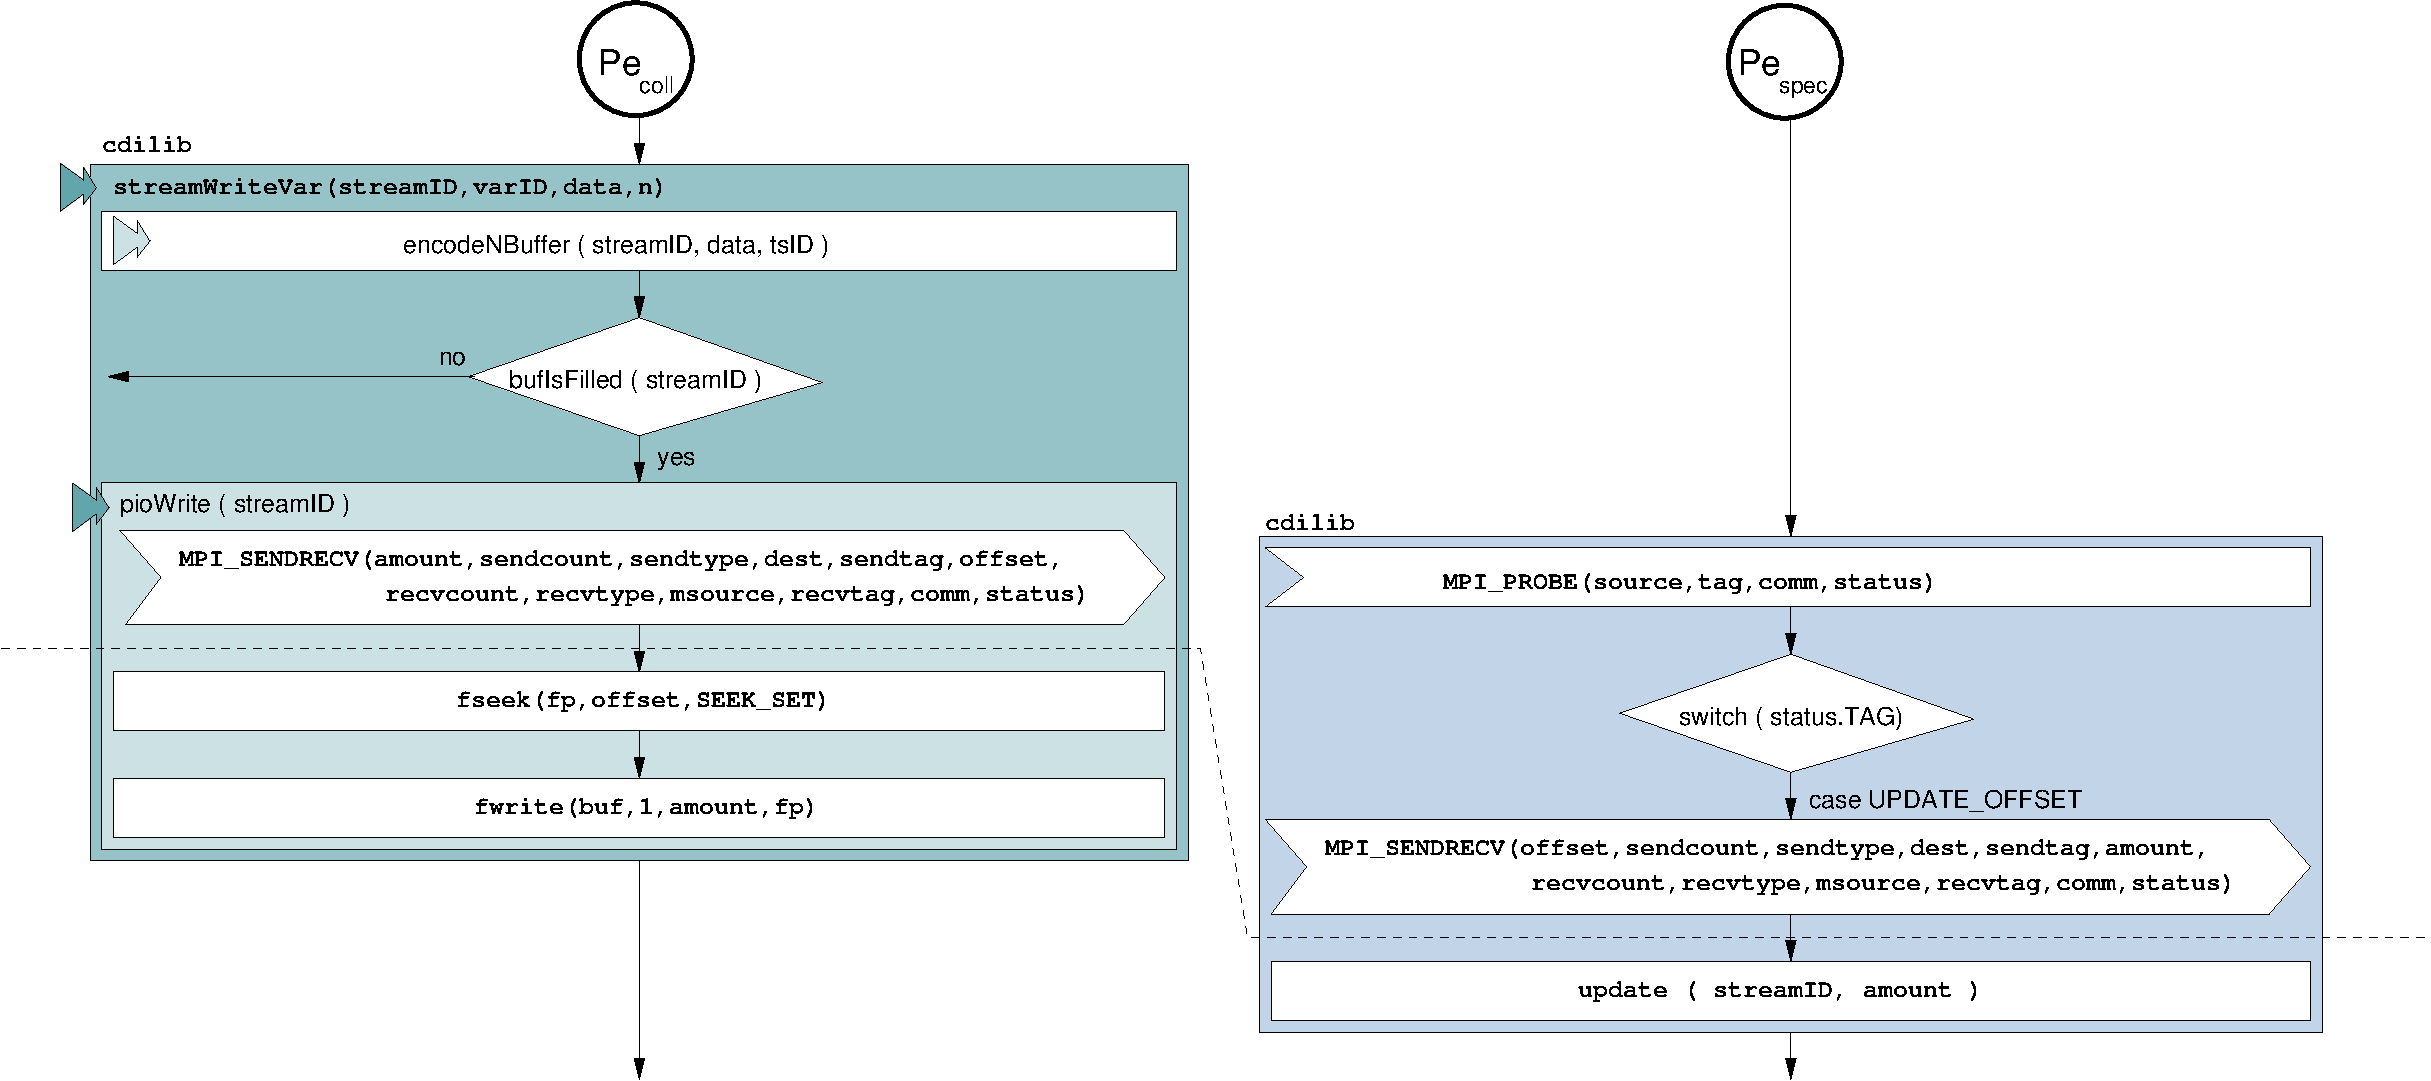
\includegraphics[scale=0.41]{../graphics/pio_fpguard.pdf}
\vspace{-10pt}
\caption{{\tt PIO\_FPGUARD}}
\vspace{-10pt}
\end{figure}
Writing a huge amount of data with a fixed file offset is a very fast
way of file writing. In this I/O mode one I/O process per physical 
node is spent to administrate the file offsets while the others do all the 
subtasks former defined for the parallel I/O. The functionality of this
collaboration is similar to
{\tt PIO\_WRITER}. Originating from {\htmlref{\tt pioInit}{pioInit}} the 
process with the highest rank calls a backend server 
function in which it is busy waiting 
for messages. The collecting I/O processes 
get data from the calculating model processes via {\tt MPI} RMA communication. 
The data is encoded, compressed and buffered. 
If the buffer is filled, the collector 
sends the count of the contained data to the ``file pointer guard'' and gets a 
file offset back. With the received offset the collector writes the data to 
file using {\tt C} standard
\texttt{fwrite} and goes on with his job. One message per collecting process 
is tagged with the finalize command. All other messages needed for 
the communication between the ``file pointer guard'' and the collectors 
contain a stream identifier, a numeric value holding the amount of buffered data
respectively the file offset and a command. There are three kinds of commands:
1. offset wanted for a file that will be newly opened, 2. offset wanted for an 
open file and 3. offset wanted for a file that will be closed after writing. 

\chapter{{\pio} modules}
\label{modules}
\section{Initialize parallel I/O: {\tt pioInit}}
\index{pioInit}
\label{pioInit}
The function {\tt pioInit} initializes the parallel I/O with {\CDI}, it launches 
the {\htmlref{\tt STAGE\_DEFINITION}{STAGEDEFINITION}}. {\tt pioInit} defines 
a control object for the {\tt MPI} communicators ( see 
figure~\ref{communicators}) and triggers their 
initialization. After starting the I/O server, {\tt pioInit} receives a message 
from each I/O process, containing information about its location on a physical node 
and its function as a collector of data or a backend server. The first information 
is stored in the control object, the latter is used to construct the communicators 
for the data transfer. Furthermore, {\tt pioInit} defines and initializes an 
control object for the {\htmlref{namespace}{namespace}}s. The call {\tt pioInit} is 
collective for all 
{\tt MPI} processes using the {\CDI}. If the 
model employs the {\CDI} serially, a  
call to {\tt pioInit} has no effect. 

\subsection*{Usage}
\begin{verbatim}
   INTEGER FUNCTION pioInit ( INTEGER commGlob, INTEGER nProcsIO, 
                              INTEGER IOMode, INTEGER nNamespaces, 
                              INTEGER hasLocalFile ( nNamespaces ));
\end{verbatim}

\hspace*{4mm}\begin{minipage}[]{15cm}
\begin{deflist}{\tt IN  hasLocalFile\ }
\item[{\tt IN  commGlob}]
{\tt MPI} communicator (handle).
\item[{\tt IN  nProcsIO}]
The number of {\tt MPI} processes that shall be used for I/O.
\item[{\tt IN  IOMode}]
The mode for the I/O. Valid I/O modes are {\htmlref{\tt PIO\_NONE}{PIONONE}}, 
{\htmlref{\tt PIO\_MPI}{PIOMPI}}, {\htmlref{\tt PIO\_WRITER}{PIOWRITER}}, 
{\htmlref{\tt PIO\_ASYNCH}{PIOASYNCH}} and 
{\htmlref{\tt PIO\_FPGUARD}{PIOFPGUARD}}.
\item[{\tt IN  nNamespaces}]
The number of used {\htmlref{namespace}{namespace}}s on the model side.
\item[{\tt IN  hasLocalFile}]
A logical array with size {\tt nNamespaces} indicating whether the model 
processes write locally or let the I/O server write.
\end{deflist}
\end{minipage}

\subsection*{Result}
Upon successfull completion {\tt pioInit} returns a {\tt FORTRAN} handle to a 
{\tt MPI} communicator including only the calculating model processes.

\subsection*{Errors}
If an error occurs, {\tt pioInit} cleans up, finalizes {\tt MPI} and exits the 
whole program.

\smallskip

The arguments of {\tt pioInit} subject to some constraints. 
\smallskip

\hspace*{4mm}\begin{minipage}[]{15cm}
\begin{deflist}{\tt nProcsIO\ }
\item[{\tt commGlob}]
\begin{itemize}
\item[]
has to be a valid handle to a {\tt MPI} communicator whose group 
includes all processes that will work on the {\CDI} resources.
\end{itemize}
\item[{\tt nProcsIO}]
\begin{itemize}
\item[]$==1$ per physical node, if {\tt IOMode} $==$ 
{\htmlref{\tt PIO\_NONE}{PIONONE}},
\item[]$<=$ {\tt sizeGlob} $/ 2$ \ otherwise, with {\tt sizeGlob} $=$ number 
of processes in {\tt commGlob},
\item[]$>= 2$ per physical node, if {\tt IOMode} $\in \{$ 
{\htmlref{\tt PIO\_WRITER}{PIOWRITER}}, 
{\htmlref{\tt PIO\_ASYNCH}{PIOASYNCH}}, 
{\htmlref{\tt PIO\_FPGUARD}{PIOFPGUARD}}$\}$.
\end{itemize} 
\end{deflist}
\end{minipage} 

\subsection*{Example}
Here is an example using {\htmlref{\tt pioInit}{pioInit}} to start parallel I/O 
in {\htmlref{\tt PIO\_NONE}{PIONONE}} mode.

\begin{lstlisting}[language=Fortran, backgroundcolor=\color{zebg}, 
basicstyle=\footnotesize, label=control]

  INCLUDE 'cdi.inc'
  INCLUDE 'mpif.h'
       ...
  INTEGER commModel, error
	...
  CALL MPI_INIT ( error )
       ...
  ! Initialize asynchronous I/O with CDI
  ! Definition stage for CDI resources
  commModel = pioInit ( MPI_COMM_WORLD, 1, PIO_NONE, 1, (/ 0 /))
	...
  CALL MODELRUN ( commModel )
       ...
  ! End cleanup stage for CDI resources
  ! Finalize asynchronous I/O with CDI
  CALL pioFinalize ()
	...
  CALL MPI_FINALIZE ( error )

\end{lstlisting}

\section{Finalize parallel I/O: {\tt pioFinalize}}
\index{pioFinalize}
\label{pioFinalize}
The function {\tt pioFinalize} finalizes the parallel I/O. It cleans up the 
{\htmlref{namespace}{namespace}}s and sends a message to the collector processes 
to close down the I/O server. The buffers and windows which where needed for 
{\tt MPI} RMA are deallocated. At last {\tt pioFinalize} frees the {\tt MPI} 
communicators ( see figure~\ref{communicators} ) 
 and destroys the control object. The call {\tt pioFinalize} is collective for all 
model processes having invoked {\htmlref{\tt pioInit}{pioInit}}. If the 
model employs the {\CDI} serially, a  
call to {\tt pioFinalize} has no effect.   

\subsection*{Usage}
\begin{verbatim}
   SUBROUTINE pioFinalize ();
\end{verbatim}
\section{Notify the end of the definition stage: {\tt pioEndDef}}
\index{pioEndDef}
\label{pioEndDef}
The end of the definition stage for the {\CDI} resources in a 
{\htmlref{namespace}{namespace}} is 
marked with a call to {\tt pioEndDef}. {\tt pioEndDef} changes the state of 
the active {\htmlref{namespace}{namespace}} to 
{\htmlref{\tt STAGE\_TIMELOOP}{STAGETIMELOOP}}. 
During this stage, a new 
definition of a {\CDI} object as well as deletion or changing of members of 
known objects in the active {\htmlref{namespace}{namespace}} will lead to an error 
and shut the program down. There is one 
exception: To write files for a defined variable list individually for 
disjunct time intervalls the three calls
\begin{itemize} 
\item {\tt SUBROUTINE streamClose ( streamID\_1 )}, 
\item {\tt INTEGER FUNCTION streamOpenWrite ( filename, filetype )} and 
\item {\tt SUBROUTINE streamDefVlist ( streamID\_2, vlistID\_1 )} 
\end{itemize}
can be used once at the beginning of a timestep, one time for each stream. When 
used with remote writing in this stage, these subprogram effect the local {\CDI} 
resources but not 
the local file system. The calls are encoded and buffered in the 
{\tt MPI} window buffer to be fetched by the collector processes. You can find a 
flowchart of a timestep on model and collecting I/O processes in figure~\ref{timestep}.
\smallskip 

{\tt pioEndDef} balances the load of the variable data among the data collecting 
I/O server and stores a mapping 
in the variables {\CDI} resource. Among the model processes {\tt pioEndDef} 
decomposes the variable in rank order, laid-out in linear memory as needed 
for the file output. An index 
array with offset and chunk is also written to the variables resource. With this 
result and the information about the decomposition for the model calculation 
it defines I/O transposition templates that will be used while writing the data. 
{\tt pioEndDef} copies the {\CDI} 
object array to a buffer and sends it to the collecting I/O server for them to 
possess the same resource handles. \smallskip

{\tt pioEndDef} calculates the memory requirement for the {\tt MPI} windows and 
buffers needed for RMA out of the dimensions stored in the {\CDI} resources. 
As a last step it allocates the buffers and creates the {\tt MPI} windows.  If 
the model uses the {\CDI} serially, a call to {\tt pioEndDef} has no effect. 

\subsection*{Usage}
\begin{verbatim}
   SUBROUTINE pioEndDef ();
\end{verbatim}

\section{Notify the end of the timestepping stage: {\tt pioEndTimestepping}}
\index{pioEndTimestepping}
\label{pioEndTimestepping}
With the function {\tt pioEndTimestepping} the end of the time integration 
is notified. \\
{\tt pioEndTimestepping} sets the state of the active 
{\htmlref{namespace}{namespace}} 
to {\htmlref{\tt STAGE\_CLEANUP}{STAGECLEANUP}}. In this stage it is possible 
to clean up the {\CDI} 
resources. There is no transfer of data or subprogram calls anymore, an attempt 
will lead to an error and shuts the whole program down. If the model uses the 
{\CDI} serially, a call to {\tt pioEndTimestepping} has no effect.

\subsection*{Usage}
\begin{verbatim}
   SUBROUTINE pioEndTimestepping ();
\end{verbatim}

\section{Move data to the collecting I/O server: {\tt pioWriteTimestep}}
The subroutine {\tt pioWriteTimestep} exposes the {\tt MPI} windows to the 
data collecting I/O server. They start to move the data from the {\tt MPI} 
window buffers of the calculating model processes to their own memory while 
the model processes can go on doing their job. The buffers contain the encoded 
subprogram calls and the variable data written by calls to {\tt streamClose}, 
{\tt streamOpenWrite}, {\tt streamDefVlist} and {\tt streamWriteVar}. If the 
model uses the {\CDI} serially, a call to\\
 {\tt pioWriteTimestep} has no effect. 

\subsection*{Usage}
\begin{verbatim}
SUBROUTINE pioWriteTimestep ( INTEGER tsID, INTEGER vdate, INTEGER vtime );
\end{verbatim}

\hspace*{4mm}\begin{minipage}[]{15cm}
\begin{deflist}{\tt IN  vdate\ } 
\item[{\tt IN  tsID}]
Timestep identifier
\item[{\tt IN  vdate}]    
Verification date (YYYYMMDD)
\item[{\tt IN  vtime}]
Verification time (hhmmss)
\end{deflist}
\end{minipage}


\subsection*{Example}
\begin{lstlisting}[language=Fortran, backgroundcolor=\color{zebg}, 
basicstyle=\footnotesize, label=model]

  INCLUDE 'cdi.inc'
  INCLUDE 'mpif.h'
       ...
  SUBROUTINE MODELRUN ( commModel )

    INTEGER streamID, vlistID, varID, tfID, ntf, tsID, nts, vdate, vtime

    ! Definition stage for CDI resources
    streamID = streamOpenWrite ( filename, filetype )
       ...
    CALL streamDefVlist(streamID, vlistID)
    
    ! End definition stage for CDI resources,
    CALL pioEndDef ()
 
    ! Timestepping stage
    DO tfID = 0, ntf-1
      IF ( tfID ) THEN
        CALL streamClose ( streamID )
	streamID = streamOpenWrite ( filename[tfID], filetype )
	CALL streamDefVlist ( streamID, vlistID )
      ENDIF 

      DO tsID = 0, nts-1
          ...
        CALL streamWriteVar(streamID, varID, varData, nmiss)
      
        ! Expose encoded and buffered subroutine calls and data 
	! to remote memory access by collecting I/O server.
        CALL pioWriteTimestep ( tsID, vdate, vtime )
      END DO
    END DO

    ! End timestepping stage
    CALL pioEndTimestepping ()

    ! Cleanup stage
    CALL streamClose(streamID)
       ...
    CALL vlistDestroy(vlistID)

  END SUBROUTINE MODELRUN

\end{lstlisting}

\section{Switch between namespaces: {\tt pioNamespaceSetActive}}
\index{pioNamespaceSetActive}
\label{pioNamespaceSetActive}
The subroutine {\tt pioNamespaceSetActive} sets the active 
{\htmlref{namespace}{namespace}} to 
the argument {\tt INTEGER IN nspID}.
The {\htmlref{namespace}{namespace}} objects are defined with the call to 
{\htmlref{\tt pioInit}{pioInit}}. A {\htmlref{namespace}{namespace}} 
object has the entries
\smallskip

% TODO: use mathmode lbrace
\hspace*{4mm}\begin{minipage}[]{15cm}
\begin{deflist}{\tt INTEGER hasLocalFile\ } 
\item[{\tt INTEGER nspID}] 
\begin{itemize}
\item[] Namespace identifier,
\end{itemize}
\item[{\tt INTEGER hasLocalFile}]
\begin{itemize}
\item[] indicating whether the {\htmlref{namespace}{namespace}} supports local 
writing,
\item[]$\in \{${\tt TRUE}, {\tt FALSE}$\}$, 
\item[]$==$ {\tt TRUE} by default,
\end{itemize}
\item[{\tt INTEGER stageCode}]
\begin{itemize}
\item[] is set by calls to the subprograms {\htmlref{\tt pioEndDef}{pioEndDef}}
 and {\htmlref{\tt pioEndTimestepping}{pioEndTimestepping}},
\item[]$\in \{${\htmlref{\tt STAGE\_DEFINITION}{STAGEDEFINITION}},{\htmlref{\tt STAGE\_TIMELOOP}{STAGETIMELOOP}},{\htmlref{\tt STAGE\_CLEANUP}{STAGECLEANUP}}$\}$, 
\item[]$==$ {\htmlref{\tt STAGE\_DEFINITION}{STAGEDEFINITION}} by default.
\end{itemize}
\end{deflist}
\end{minipage}
\smallskip

 If the model uses the {\CDI} serially, a call to {\tt pioNamespaceSetActive} 
has no effect.\\
\smallskip 

\subsection*{Usage}
\begin{verbatim}
SUBROUTINE pioNamespaceSetActive ( INTEGER nspID )
\end{verbatim}

\hspace*{4mm}\begin{minipage}[]{15cm}
\begin{deflist}{\tt IN  nspID\ } 
\item[{\tt IN  nspID}]
Namespace identifier
\end{deflist}
\end{minipage}


\section{Offset of the local I/O subvariable: {\tt pioInqVarDecoOff}}
\index{pioInqVarDecoOff}
\label{pioInqVarDecoOff}
Obsolete. 

\subsection*{Usage}
\begin{verbatim}
   INTEGER FUNCTION pioInqVarDecoOff ( INTEGER vlistID, INTEGER varID )
\end{verbatim}

\hspace*{4mm}\begin{minipage}[]{15cm}
\begin{deflist}{\tt IN  vlistID\ } 
\item[{\tt IN  vlistID}]
Variable list identifier
\item[{\tt IN  varID}]
Variable identifier
\end{deflist}
\end{minipage}

\section{Chunk of the local I/O subvariable: {\tt pioInqVarDecoChunk}}
\index{pioInqVarDecoChunk}
\label{pioInqVarDecoChunk}
Obsolete.

\subsection*{Usage}
\begin{verbatim}
   INTEGER FUNCTION pioInqVarDecoChunk ( INTEGER vlistID, INTEGER varID )
\end{verbatim}

\hspace*{4mm}\begin{minipage}[]{15cm}
\begin{deflist}{\tt IN  vlistID\ } 
\item[{\tt IN  vlistID}]
Variable list identifier
\item[{\tt IN  varID}]
Variable identifier
\end{deflist}
\end{minipage}

\chapter{Internal concepts}
\section{{\tt MPI} communicators}

\begin{figure}[H]
\centering
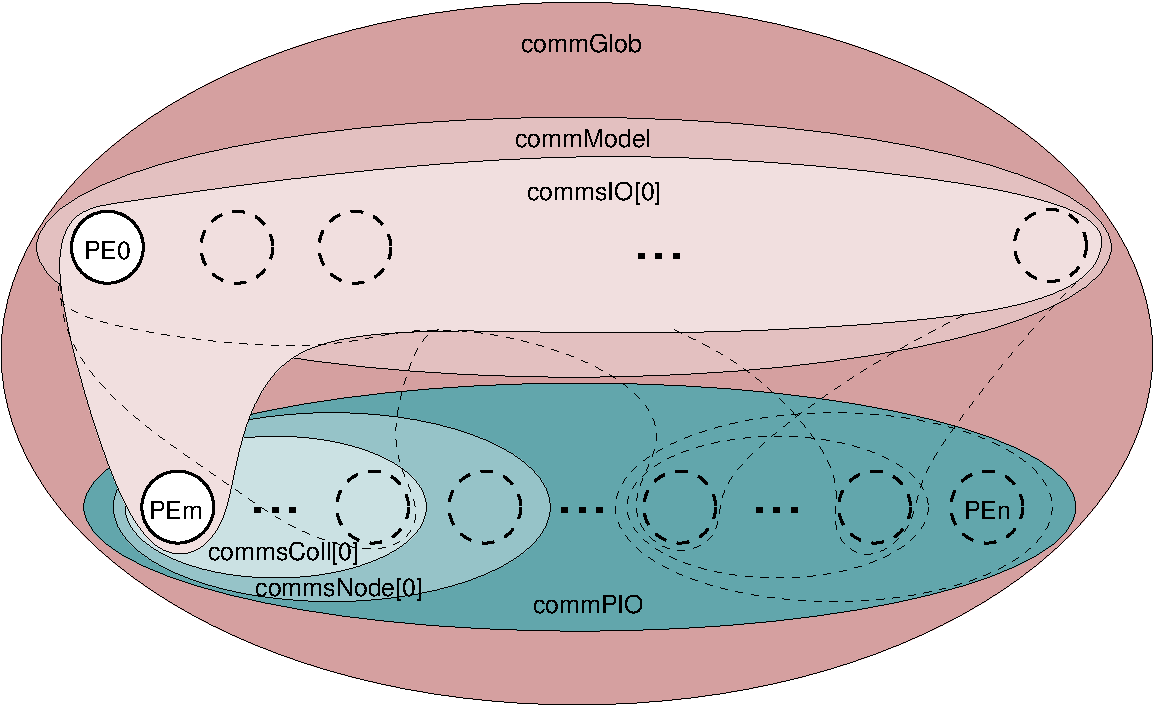
\includegraphics[scale=0.6]{../graphics/communicators.pdf}
\caption {Participation of {\tt MPI} processes in communication 
``universes''.}
\label{communicators}
\end{figure}

\section{Timestepping}

\begin{figure}[H]
\centering
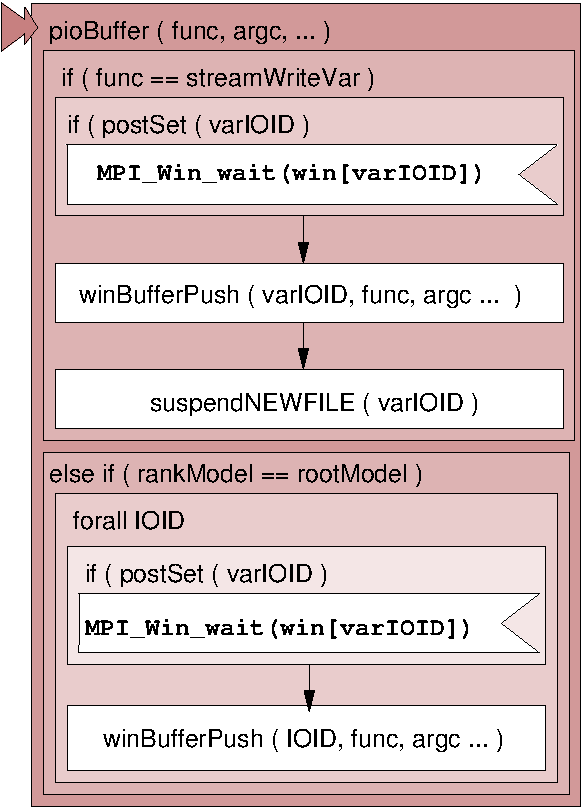
\includegraphics[scale=0.6]{../graphics/pioBuffer.pdf}
\caption {Pseudo code pioBuffer used in figure timestep {\tt tsID}}
\end{figure}

\begin{figure}[H]
\centering
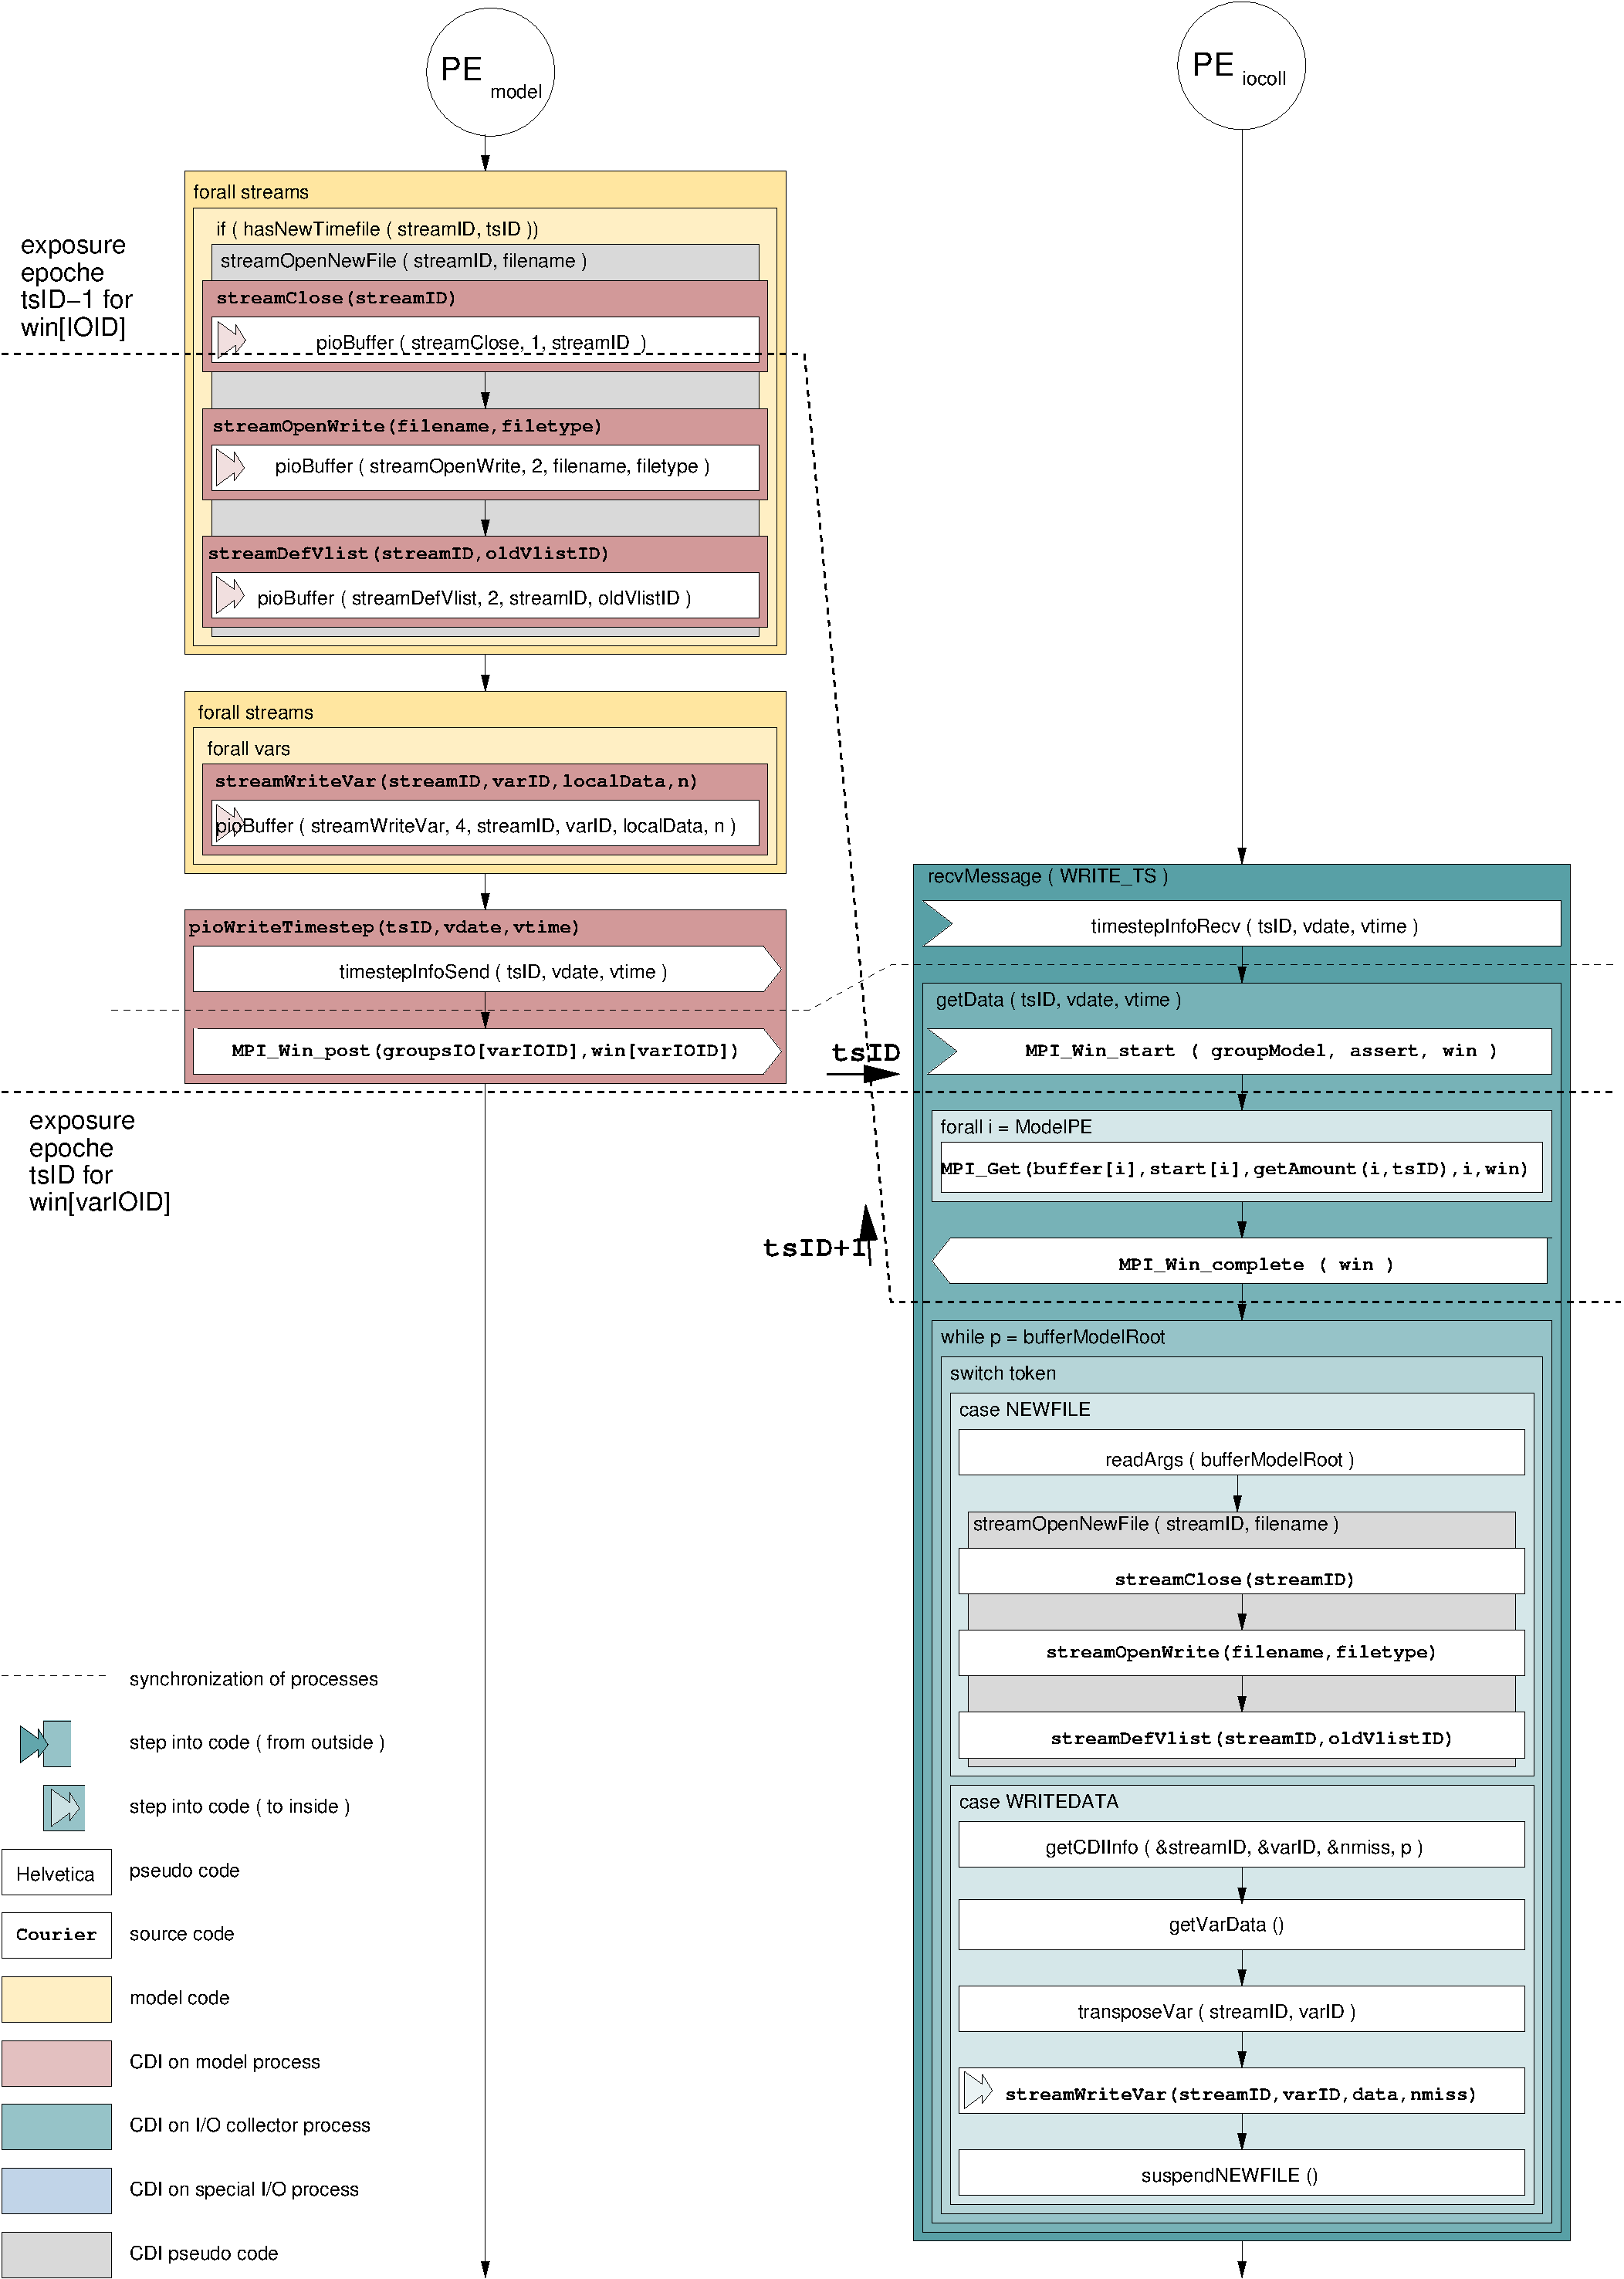
\includegraphics[scale=0.5]{../graphics/timestep.pdf}
\caption { Timestep {\tt tsID} on model and I/O collector processes.}
\index{timestep}
\label{timestep}
\end{figure}

\printindex

\end{document}